\section{ResultAnalysis}

\subsection{System Dashboard and Overview}
The front-end application, built with Streamlit, provides a real-time visualization of the database state. The System Dashboard confirms the successful ingestion and processing of the historical dataset.

\begin{figure}[h!]
\begin{center}
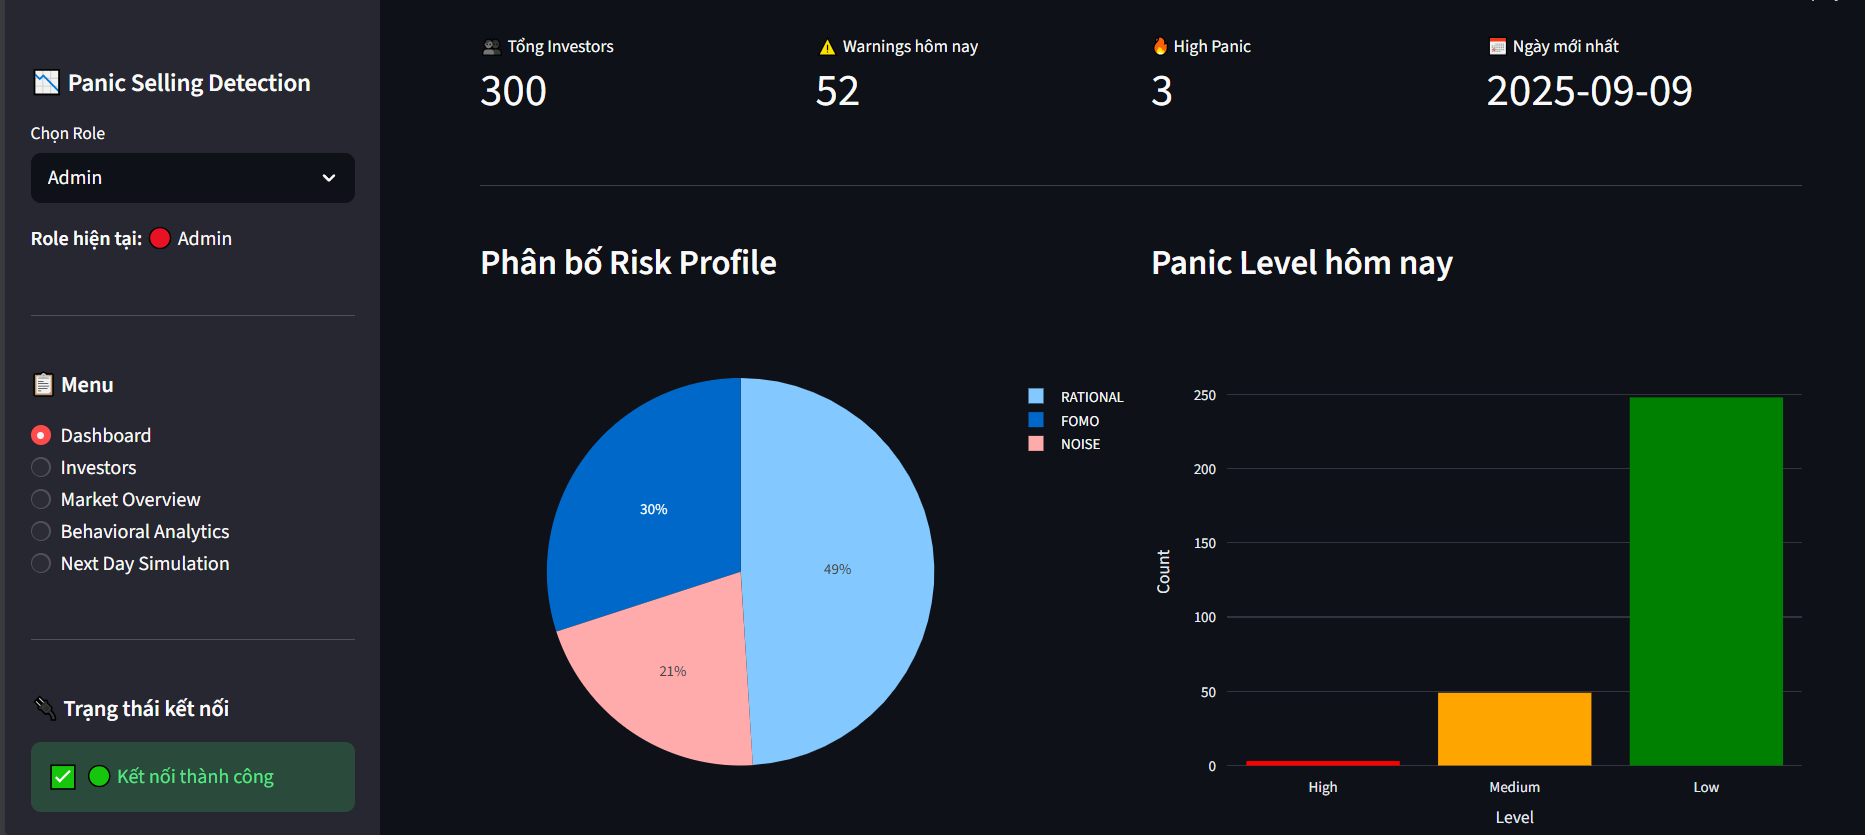
\includegraphics[width=\textwidth]{Images/dashboard.png}
\end{center}
\caption{Main System Dashboard visualizing core metrics and risk distributions.}
\end{figure}

The dashboard displays four primary metric cards:
\begin{itemize}
    \item \textbf{Total Investors:} 300 active profiles monitored.
    \item \textbf{Warnings Generated:} 52 alerts triggered specifically on 09/09/2025, confirming the \texttt{AFTER INSERT} database trigger executes correctly.
    \item \textbf{High Panic Current:} 3 investors flagged. This low number indicates the $\ge 0.6$ threshold is appropriately strict, isolating only the most severe cases rather than generating excessive noise.
    \item \textbf{Latest Observation Date:} 2025-09-09, verifying the ELT pipeline successfully advances the timeline.
\end{itemize}

The visual distribution aligns with the initial database design parameters. The pie chart displays a risk profile breakdown of RATIONAL (49\%), FOMO (30\%), and NOISE (21\%), matching the synthetic data generation configuration. The PanicLevel bar chart shows a logical right-skewed distribution: the vast majority of signals are classified as Low, a moderate portion as Medium, and a very small fraction as High.

\textbf{Role Switching (UI to Database Mapping):} 
The left sidebar includes a "Select Role" dropdown. This UI element dynamically alters the SQLAlchemy connection string to authenticate as different MySQL users (\texttt{admin\_user}, \texttt{analyst\_user}, \texttt{viewer\_user}). 
\begin{itemize}
    \item The \textbf{Admin} interface exposes all 5 pages.
    \item The \textbf{Analyst} interface restricts access to 3 pages, hiding the raw Investors and Market Overview tables.
    \item The \textbf{Viewer} interface grants access only to the Dashboard and Warning Board. It pulls data strictly from the \texttt{vw\_public\_warnings} view, ensuring \texttt{InvestorID}s remain completely masked to comply with data privacy controls.
\end{itemize}

\subsection{Warning System Results}

\begin{figure}[h!]
\begin{center}
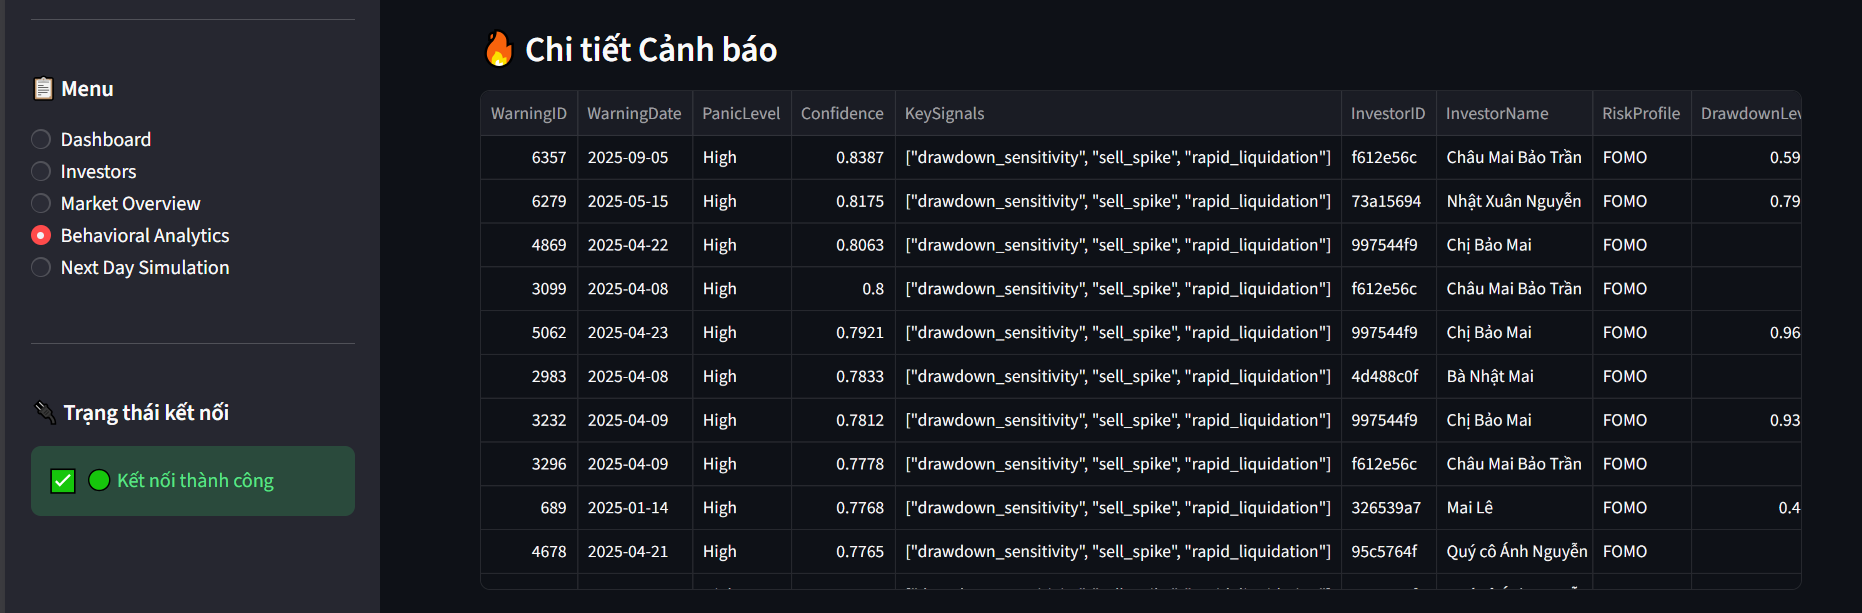
\includegraphics[width=\textwidth]{Images/warning_dashboard.png}
\end{center}
\caption{Warning Dashboard displaying high-risk investors and trigger confidence.}
\end{figure}

Analysis of the detailed warning logs reveals the efficacy of the behavioral metrics:
\begin{itemize}
    \item \textbf{Profile Correlation:} Every investor categorized under "High Panic" belongs to the FOMO group. This validates that the mathematical weighting in \texttt{fn\_panic\_score} accurately captures the specific psychological biases (high chasing bias, high loss aversion) configured during generation.
    \item \textbf{Recurrent Behavior:} Investor \texttt{f612e56c} triggers the highest confidence score (0.8387) and appears multiple times (e.g., 04/08, 04/09). This indicates a pattern of recurrent panic behavior rather than an isolated miscalculation.
    \item \textbf{Trigger Logic Verification:} The \texttt{KeySignals} JSON column for High Panic records consistently contains all three tags: \texttt{["drawdown\_sensitivity", "sell\_spike", "rapid\_liquidation"]}. This proves the JSON string concatenation logic within the database trigger evaluates all conditions correctly.
    \item \textbf{Temporal Clustering:} Warnings heavily cluster around April and September 2025. Cross-referencing these dates with the \texttt{MarketData} table confirms these periods align with widespread PANIC market regimes, demonstrating the system's sensitivity to macro-level market stress.
\end{itemize}

\subsection{Next Day Simulation Results}

\begin{figure}[h!]
\begin{center}
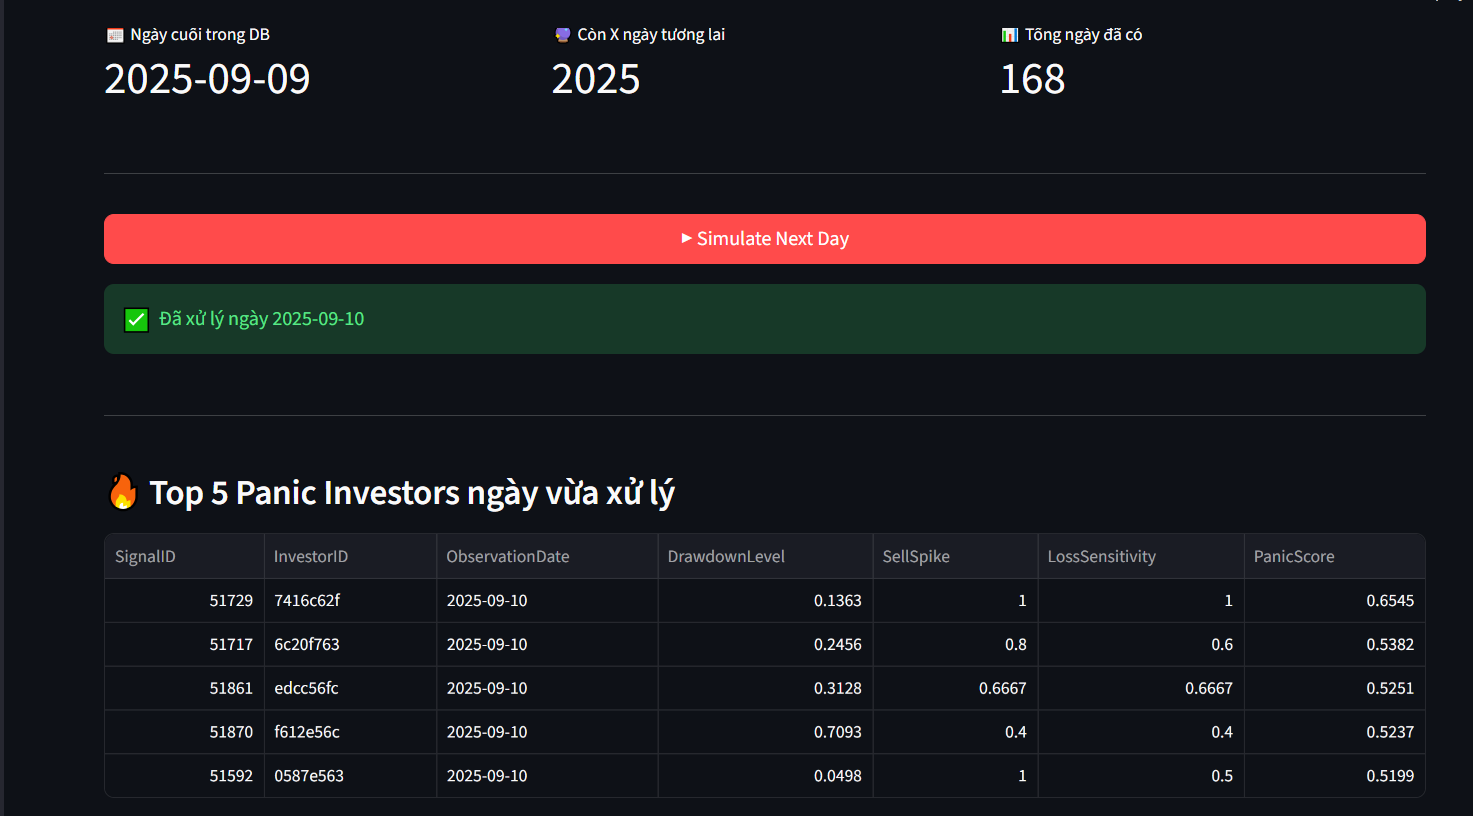
\includegraphics[width=\textwidth]{Images/next_day.png}
\end{center}
\caption{Execution interface and immediate results of the Next Day Simulation pipeline.}
\end{figure}

The Next Day module tests the system's real-time processing capabilities. Prior to execution, the database holds 168 trading days of data, with the latest record on 2025-09-09.

Upon executing the simulation for the subsequent day (2025-09-10), the application immediately returns the top 5 Panic Investors. For example, Investor \texttt{7416c62f} registers a \texttt{SellSpike = 1.0} and a \texttt{LossSensitivity = 1.0}. This signifies that 100\% of their sell orders within the 30-day window were panic-driven and executed at a loss—an indicator of extreme capital capitulation. This pushes their \texttt{PanicScore} to 0.6545, crossing the High threshold.

The results confirm the architectural integrity of the ELT design. A single user click triggers a raw data \texttt{INSERT}. Following the insert, the application issues one \texttt{CALL} statement. The entire computational sequence—evaluating 300 portfolios, calculating moving window metrics via 4 UDFs, inserting into \texttt{BehaviorSignals}, and generating JSON-formatted alerts via triggers—executes entirely within the database layer. The Python application performs zero mathematical logic, acting strictly as the presentation layer for the MySQL engine's output.